\documentclass[../main/main.tex]{subfiles}

\newdate{date}{17}{04}{2020}

\begin{document}

\chapter{Perturbation theory}

\marginpar{ \textbf{Lecture 11.} \\  \displaydate{date}. \\ Compiled:  \today.}
The preceding section described the single-particle Green's function. Unfortunately it is very difficult to know the exact Green's function because it is equivalent to know the exact solution of the Schr$\ddot{o}$dinger equation and we have to make approximations if we want to deal with the many-body problem.
To address the many-body problem we should try to evaluate the Green's function approximately by a \emph{perturbative approach}:
\begin{equation*}
  \hat{H} = \hat{H}_0 + \hat{H}_1
\end{equation*}
where we have assumed that our Hamiltonian is constituted by a non-interacting term \( \hat{H}_0  \) (supposed known) and a difficult interacting term \( \hat{H}_1  \)\footnote{In the case of free fermions we have derived both the basic properties and also the non-interacting Green's function.}. The next chapter will be devoted to present such a possible perturbative approach for evaluating in an approximate way the Green's function.

To be more precise, now we will introduce the so called \textbf{adiabatic  “switching on”} approach. \marginpar{Adiabatic “switching on” approach} The idea is that even though \( H \) is tipically time independent, we can introduce an Hamiltonian which is formally time dependent as follow:
\begin{equation*}
  \hat{H} (t) = \hat{H}_0 + + e^{-\varepsilon \abs{t} } \hat{H}_1
\end{equation*}
where \( \varepsilon \rightarrow 0^+  \) is a small positive quantity. In particular, results should not depend on the specific value of this parameter.
Hence, at time zero we will recover the full interacting system, while for very large times (both in the past and in the future) the hamiltonian tends to the simpler non-interacting hamiltonian:
\begin{equation*}
  \hat{H} (0) = \hat{H}_0 + \hat{H}_1, \qquad \hat{H} (t \rightarrow \pm \infty ) = \hat{H}_0
\end{equation*}
Let us consider the usual Schr$\ddot{o}$dinger equation:
\begin{equation*}
  \hat{H} (t) \ket{\psi _E (t)} = E(t)  \ket{\psi _E (t)}
\end{equation*}
The adiabatic “switching on” approach means that the full interacting eigenstate tends to the non interacting state for \( t \rightarrow \pm \infty \), by assuming that it is the eigenstate for the non interacting system:
\begin{equation*}
  \lim_{t \rightarrow \pm \infty } \ket{\psi _E (t)} = \ket{\Phi _E}, \qquad \hat{H}_0 \ket{\Phi _E} = E_0 \ket{\Phi _E}
\end{equation*}
Schematically, we can say that the eigenvalue goes from the non-interacting value in the past (\( t \rightarrow - \infty  \)), at \( t=0 \) becomes the eigenvalue of the full interacting system and finally for very large positive times (\( t \rightarrow +\infty  \)) it returns to the non-interacting system.

For a more convenient perturbative evaluation of the Green's function it is useful to consider different “pictures” of quantum mechanics. Indeed, in order to perform this perturbative approach it is more convenient to use a picture called “interaction picture” rather than the standard Schr$\ddot{o}$dinger one.

\subsection{Pictures of quantum mechanics}

\subsubsection{Schr$\pmb{\ddot{o}}$dinger picture}
The usual elementary description of quantum mechanics assumes that the state vectors are time dependent, wherears the operators are time independent and are constructed by the familiar rules from the corresponding classical quantities. The Schr$\ddot{o}$dinger equation therefore takes the form
\begin{equation}
  i \hbar \pdv{}{t} \ket{\psi _S (t)} = \hat{H}  \ket{\psi _S (t)}, \qquad \hat{H} = \hat{H}_0 + \hat{H}_1
  \label{eq:11_1}
\end{equation}
where \( \hat{H}  \) is assumed to have no explicit time dependence.
Since Eq.\eqref{eq:11_1} is a first-order differential equation, the initial state at \( t_0 \) determines the subsequent behaviour, and a formal solution is readily obtained by writing
\begin{equation}
  \ket{\psi _S (t)} = e^{-i \hat{H} (t-t_0)/\hbar  } \ket{\psi _S (t_0)}
  \label{eq:11_2}
\end{equation}
Here the exponential of an operator is defined in terms of its power series expansion. Furthermore, \( \hat{H}  \) is hermitian so that the exponential represents a unitary operator. Given the solution to the Schr$\ddot{o}$dinger equation at the time \( t_0 \), the unitary transformation in Eq.\eqref{eq:11_2} generates the solution at time \( t \).

\subsubsection{Heisenberg picture}
The state vector in the Heisenberg picture is defined as
\begin{equation}
  \ket{\psi _H (t)} = e^{i \hat{H} t/\hbar  } \ket{\psi _S (t)}
  = \ket{\psi _S (0)}
\end{equation}
where in the second step we used Eq.\eqref{eq:11_2} (at \( t_0=0 \)) obtaining that the state vector is time independent. The generic operator in the Heisenberg picture can be written as:
\begin{equation}
  \hat{O}_H (t) = e^{i \hat{H}t/\hbar  } \hat{O}_S  e^{-i \hat{H}t/\hbar  }
\end{equation}
which instead depends on time.


\subsubsection{Interaction picture}
Let us suppose\footnote{The interaction picture has been implicitely used when we have played with the non-interacting Green's function \( G_0 \), even if we have not called that as interaction picture.} to have a general time independent operator \( \hat{O}_S  \), as in the usual Schr$\ddot{o}$dinger picture.
In the interaction picture we define a generic operator as follow:
\begin{equation}
  \hat{O}_I (t) \equiv e^{i \hat{H}_0 t / \hbar  }  \hat{O}_S e^{-i \hat{H}_0 t / \hbar  }
  \label{eq:11_3}
\end{equation}
where the time dependence is essentially driven by the exponential factor, while \( H_0 \) is the non-interacting hamiltonian.

Clearly, different “pictures” of quantum mechanics must be physically equivalent. It means that the matrix element that we compute by using for instance the interaction picture, must be equal to the corresponding matrix element obtained using the Schr$\ddot{o}$dinger picture:
\begin{equation*}
  \bra{\psi _I (t)} \hat{O}_I \ket{\psi _I (t)}
  = \bra{\psi _I (t)} e^{i \hat{H}_0 t / \hbar  }  \hat{O}_S e^{-i \hat{H}_0 t / \hbar  } \ket{\psi _I (t)}
  =  \bra{\psi _S (t)} \hat{O}_S \ket{\psi _S (t)}
\end{equation*}
It must be:
\begin{equation*}
  e^{-i \hat{H}_0 t / \hbar  } \ket{\psi _I (t)} = \ket{\psi _S (t)}
\end{equation*}
which relate the state vector in the interaction picture with the state vector in the Schr$\ddot{o}$dinger picture. Clearly, if we invert this relation we get the state vector in the interaction picture:
\begin{equation}
  \ket{\psi_I (t) } =   e^{i \hat{H}_0 t / \hbar  } \ket{\psi _S (t)}
  \label{eq:11_4}
\end{equation}
and since \( \hat{H} _0 \) is an hermitian operator, this is a unitary transformation.
In particular, we note that in the interaction picture the operators and the state vectors both depend on time, but the time-dependence of the operators is particularly simple.


\begin{table}[h!]
  \centering
\begin{tabular}{lll}
  \toprule
  \textbf{Picture}  & \textbf{State vector} & \textbf{Operator} \\
  \midrule
  \textbf{Schr$\pmb{\ddot{o}}$dinger} & \( \scriptstyle {\ket{\psi _S (t)} = e^{-i \hat{H}t/\hbar  } \ket{\psi _S (0)} } \) & \( \scriptstyle {\hat{O}_S } \) \\
   & depends on time & time-independent \\
  \midrule
  \textbf{Heisenberg}  & \( \scriptstyle{ \ket{\psi _H (t)} = e^{i \hat{H} t/\hbar  } \ket{\psi _S (t)} = \ket{\psi _S (0)} } \) & \(  \scriptstyle{ \hat{O}_H (t) = e^{i \hat{H}t/\hbar  } \hat{O}_S  e^{-i \hat{H}t/\hbar  }  } \)\\
  & time-independent & depends on time \\
  \midrule
  \textbf{Interaction}  & \( \scriptstyle{  \ket{\psi_I (t) } =   e^{i \hat{H}_0 t / \hbar  } \ket{\psi _S (t)} }  \) & \( \scriptstyle{  \hat{O}_I (t) \equiv e^{i \hat{H}_0 t / \hbar  }  \hat{O}_S e^{-i \hat{H}_0 t / \hbar  } }\) \\
  & depends on time & \( \substack{ \text{depends on time} \\  \text{but the time dependence is simple} }  \) \\
   \bottomrule
\end{tabular}
\caption{Summary of the different pictures for the quantum mechanical description of the system. Let us note that the time-dependence of the interaction operator is very simple, because it does not depend on the full hamiltnonian but just on the easy non-interacting part \( \hat{H}_0  \). The general operator in the Heisenberg picture as a complicated time-dependence in terms of the full interacting hamiltonian.}
\end{table}


\noindent In addition, it is easy to show that the three different pictures coincide at \( t=0 \):
\begin{subequations}
\begin{align}
  \ket{\psi _H} = \ket{\psi _S (0)} = \ket{\psi _I (0)}  \\
  \hat{O}_S = \hat{O}_H (0) = \hat{O} _I (0)
\end{align}
\end{subequations}

Let us find the equation of motion of the state vector in the interaction picture: \marginpar{Interaction picture: equation of motion}
\begin{equation*}
\begin{split}
  i \hbar \pdv{}{t} \ket{\psi _I (t)} &= - \hat{H}_0 e^{i \hat{H}_0 t/ \hbar  } \ket{\psi _S (t)} +  e^{i \hat{H}_0 t/ \hbar  } \mathcolorbox{green!20}{i \hbar \pdv{}{t} \ket{\psi _S (t)}}    \\
  &\overset{\eqref{eq:11_1}}{=}  - \cancel{\hat{H}_0  e^{i \hat{H}_0 t/ \hbar  } \ket{\psi _S (t)} }
  + e^{i \hat{H}_0 t/ \hbar  } \mathcolorbox{green!20}{\qty[ \cancel{\hat{H}_0} + \hat{H}_1  ] \ket{\psi _S (t)}}
\end{split}
\end{equation*}
where we can delete the terms because \( \hat{H}_0  \) and \( e^{i \hat{H}_0 t/\hbar  }  \) commute.
Thus we obtain:
\begin{equation*}
\begin{split}
  i \hbar \pdv{}{t} \ket{\psi _I (t)} &= e^{i \hat{H}_0 t/ \hbar  } \hat{H}_1 \ket{\psi _S (t)}  = \qty(e^{i \hat{H}_0 t/ \hbar  } \hat{H}_1 e^{-i \hat{H}_0 t/ \hbar  }) \qty(e^{i \hat{H}_0 t/ \hbar  } \ket{\psi _S (t)} )  \\
  &= \hat{H}_{I_1} (t)  \ket{\psi _I (t)}
\end{split}
\end{equation*}
We can conclude that the time dependent state vector in the interaction picture satisfies a Schr$\ddot{o}$dinger like equation with the difference that with respect to the ordinary Schr$\ddot{o}$dinger equation there is \emph{only} the interaction part of the hamiltonian \( \hat{H}  \):\footnote{More or less this is the reason of the name, because we obtain an equation of motion with only the difficult perturbation part.}
\begin{equation}
  i \hbar \pdv{}{t} \ket{\psi _I (t)} = \hat{H}_{I_1} (t)  \ket{\psi _I (t)}
\end{equation}

In order to solve in practice the equation of motion in the interaction picture it is convenient to define a unitary operator \( \hat{U} (t,t_0)  \) such that it determines the time-evolution from \( t_0 \) to \( t \) of a state vector:
\begin{equation}
  \ket{\psi _I (t)} = \hat{U} (t,t_0) \ket{\psi _I (t_0)}
  \label{eq:11_6}
\end{equation}
Formally we can write \( \hat{U} (t,t_0)  \) as follows:
\begin{equation}
\begin{split}
  \ket{\psi _I (t)} &= e^{i \hat{H}_0 t/ \hbar  } \ket{\psi _S (t)}
  \overset{\eqref{eq:11_2}}{=}   e^{i \hat{H}_0 t/ \hbar  } e^{-i \hat{H} (t-t_0)/ \hbar  } \ket{\psi _S (t_0)} \\
  &= \mathcolorbox{yellow!40}{\qty( e^{i \hat{H}_0 t/ \hbar  }  e^{-i \hat{H} (t-t_0)/ \hbar  }   e^{-i \hat{H}_0 t_0/ \hbar  }   )}  \ket{\psi _I (t_0)} \\
  &= \hat{U} (t,t_0) \ket{\psi _I (t_0)}
\end{split}
\label{eq:11_5}
\end{equation}
We can easily demonstrate that:
\begin{itemize}
\item \( \hat{U} (t,t_0)  \) is an \textbf{unitary operator}:
\begin{equation*}
  \hat{U} ^\dag (t,t_0)\hat{U} (t,t_0) = \mathbb{1} \quad \Rightarrow \hat{U} ^\dag  (t,t_0) = \hat{U}^{-1}  (t,t_0)
\end{equation*}
\item \( \hat{U} (t,t_0) \) has the \textbf{group property}:
\begin{equation*}
  \hat{U} (t,t_0) = \hat{U} (t,t_1)\hat{U} (t_1,t_0)
\end{equation*}
\item \( \hat{U} (t,t_0) \) is coherent with the notion of \textbf{evolution operator}:
\begin{equation*}
  \hat{U} (t_0,t_0) = \mathbb{1} \quad \Rightarrow \hat{U} (t_0,t) \hat{U} (t,t_0) = \mathbb{1}
\end{equation*}
which implies that
\begin{equation*}
    \hat{U} ^\dag (t,t_0) = \hat{U} (t_0,t)
\end{equation*}
\end{itemize}

Altough Eq.\eqref{eq:11_5} is the formal solution to the problem posed by Eq.\eqref{eq:11_6}, it is not very useful for computational purposes because it is very complicated. Indeed, \( \hat{H}  \) and \( \hat{H}_0  \) do not commute and the total order of these operators must be preserved.

It is more convenient to construct an integral equation for \( \hat{U}  \) (of course involving the interaction part of the interaction picture, \( \hat{H}_{I_1}  \)), which can then be solved by iteration.
This integral equation can be easily obtained by remembering the equation of motion for the state vector in the interaction picture:
\begin{equation*}
\begin{split}
   i \hbar \pdv{}{t} \ket{\psi _I (t)} &= \hat{H}_{I_1} (t)  \ket{\psi _I (t)}  \\
   \Rightarrow
   i \hbar \pdv{}{t} \qty( \hat{U} (t,t_0)   \ket{\psi _I (t_0)})
   &= \hat{H}_{I_1} (t) \hat{U} (t,t_0) \ket{\psi _I (t_0)}
\end{split}
\end{equation*}
Since this differential equation must hold for any (time-independent) \( \ket{\psi _I (t_0)} \) factor, as a consequence the time evolution operator \( \hat{U}  \) must satisfies itself this differential equation:
\begin{equation*}
  i \hbar  \pdv{}{t} \hat{U} (t,t_0) = \hat{H}_{I_1} (t) \hat{U} (t,t_0)
\end{equation*}
Changing \( t \rightarrow t' \) and integrating the equation from \( t_0 \) to \( t \):
\begin{equation*}
  \int_{t_0}^{t} \dd[]{t'} i \hbar \pdv{}{t'} \hat{U} (t',t_0)
  = \int_{t_0}^{t} \dd[]{t'} \hat{H}_{I_1} (t') \hat{U} (t',t_0)
\end{equation*}
Clearly the left hand integral is quite easy:
\begin{equation*}
  i \hbar \qty[ \hat{U} (t,t_0) - \underbrace{\hat{U} (t_0,t_0)}_{=\mathbb{1}}   ]
  =  \int_{t_0}^{t} \dd[]{t'} \hat{H}_{I_1} (t') \hat{U} (t',t_0)
\end{equation*}

\begin{equation}
  \hat{U} (t,t_0) = 1 - \frac{i}{\hbar } \int_{t_0}^{t} \dd[]{t'} \hat{H}_{I_1} (t') \hat{U} (t',t_0)
\end{equation}
The last integral is complicated because it contains the \( \hat{U}  \) operator both outside and inside the integral.
Clearly, the time independent variable \( t \) appears as the \emph{upper limit} in the integral. Thus, if in place of the \( \hat{U}  \) operator (inside the integral) we had a c-number, it would be a “\textbf{Volterra integral equation}” which may be solved by \emph{iteration} (and the solution is guaranteed to converge); in our case \( \hat{U}  \) is an operator, but we try to solve the equation by iteration always mantaining the \emph{proper order} of the operators during all the derivation. At the end we should check that we found a reasonable result, because there is no assurance that the present operator equation has the same properties.

By iteration means that we can interpret the interaction part \( \hat{H}_{I_1}  \) as a small perturbation:
\begin{itemize}
\item at order \( 0 \): \( \hat{U}^{(0)} (t,t_0) = \mathbb{1}  \)\footnote{Because if we neglect the term containing the \(\hat{H}_{I_1}\) in the integral equation, we have left with just \( \mathbb{1} \))};
\item at order \( 1 \): \( \hat{U}^{(1)} (t,t_0) = \mathbb{1} - \frac{i}{\hbar } \int_{t_0}^{t} \dd[]{t_1} \hat{H}_{I_1} (t_1) \mathbb{1}    \);
\item at order \( 2 \):
\begin{equation*}
\begin{split}
  \hat{U}^{(2)} (t,t_0) &= \mathbb{1} - \frac{i}{\hbar } \int_{t_0}^{t} \dd[]{t_1} \hat{H}_{I_1} (t_1) \hat{U}^{(1)} (t_1,t_0) \\
  &= \mathbb{1} - \frac{i}{\hbar } \int_{t_0}^{t} \dd[]{t_1} \hat{H}_{I_1} (t_1)
  -\frac{1}{\hbar^2 } \int_{t_0}^{t} \dd[]{t_1} \hat{H}_{I_1} (t_1) \int_{t_0}^{t_1} \dd[]{t_2} \hat{H}_{I_1} (t_2)
\end{split}
\end{equation*}
\item at order \( n \):
\begin{equation}
  \hat{U}^{(n)} (t,t_0) = \mathbb{1} - \frac{i}{\hbar } \int_{t_0}^{t} \dd[]{t_1} \hat{H}_{I_1} (t_1) \hat{U}^{(n-1)} (t_1,t_0)
\end{equation}
\end{itemize}

In order to proceed, let us focus on the double integral inside the expansion at order \( 2 \). This term can be rweritten as:
\begin{equation}
\begin{split}
  \int_{t_0}^{t} \dd[]{t_1} \hat{H}_{I_1} (t_1) \int_{t_0}^{t_1} \dd[]{t_2} \hat{H}_{I_1} (t_2) &=
  \frac{1}{2} \mathcolorbox{red!40}{\int_{t_0}^{t} \dd[]{t_1} \int_{t_0}^{t_1} \dd[]{t_2}} \hat{H}_{I_1} (t_1)  \hat{H}_{I_1} (t_2) +  \\
  &+ \frac{1}{2}  \mathcolorbox{blue!20}{ \int_{t_0}^{t} \dd[]{t_2} \int_{t_2}^{t} \dd[]{t_1}}  \hat{H}_{I_1}(t_1) \hat{H}_{I_1} (t_2)
\end{split}
\label{eq:11_7}
\end{equation}
since the last term on the right is just obtained by reversing the order of the integrations, as illustrated in Fig.\ref{fig:11_1}.
\begin{itemize}
\item The first integration order in red (Eq.\eqref{eq:11_7}) means that first we fix \( t_1 \); then \( t_2 \) goes from \( t_0 \) to \( t_1 \). After that \( t_1 \) goes from \( t_0 \) to \( t \).
\item In the second integral, for a given \( t_2 \), \( t_1 \) goes from \( t_2 \) to \( t \); then \( t_2 \) goes from \( t_0 \) to \( t \).
\end{itemize}
So you cover exactly the same integration region, what is changed is just the order of integration.


\begin{figure}[h!]
\centering
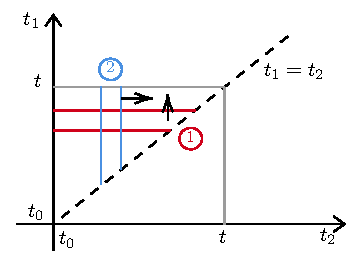
\includegraphics[width=0.5\textwidth]{../lessons/11_image/1.pdf}
\caption{\label{fig:11_1} Integration regions for second order-term \( \hat{U} (t,t_0)  \). The integration regions are the same, just the order of the integrations is reversed. In particular, the region \( 1 \), in red, corresponds to the red integral in Eq.\eqref{eq:11_7}, while the region \( 2 \) to the second integral.}
\end{figure}

By interchanging the integration dummy variables in the second integral (\( t_1 \rightarrow t_2, t_2 \rightarrow t_1 \)) we have:
\begin{equation*}
  \frac{1}{2}   \int_{t_0}^{t} \dd[]{t_1} \int_{t_1}^{t} \dd[]{t_2} \hat{H}_{I_1}(t_2) \hat{H}_{I_1} (t_1)
\end{equation*}
and recombining it with the first integral
\begin{equation*}
\begin{split}
  \int_{t_0}^{t} \dd[]{t_1} \int_{t_0}^{t_1} \dd[]{t_2}  \hat{H}_{I_1} (t_1) \hat{H}_{I_1} (t_2) =
  \frac{1}{2} \int_{t_0}^{t} \dd[]{t_1} \int_{t_0}^{t} \dd[]{t_2}
  & \Big[ \hat{H}_{I_1} (t_1) \hat{H}_{I_1} (t_2) \Theta (t_1 - t_2) + \\
  &+ \hat{H}_{I_1} (t_2) \hat{H}_{I_1} (t_1) \Theta (t_2 - t_1)  \Big]
\end{split}
\end{equation*}
Now (this is the exciting conclusion) we can replace the expression on the square parenthesis with just a time ordered product of the sequence of the two hamiltonian:
\begin{equation}
    \int_{t_0}^{t} \dd[]{t_1} \int_{t_0}^{t_1} \dd[]{t_2}  \hat{H}_{I_1} (t_1) \hat{H}_{I_1} (t_2)
    = \frac{1}{2!} \int_{t_0}^{t} \dd[]{t_1} \int_{t_0}^{t} \dd[]{t_2}
    T \qty[ \hat{H}_{I_1} (t_1) \hat{H}_{I_1} (t_2)  ]
\end{equation}
Note that the \( \hat{H}_{I_1}  \) do not necessarily commute at different times thus the proper order of the operators must be mantained. Furthermore, having introduced the time-ordered product, we have some hope that we there is a connection with the Green's function.
It is a consistent definition also for fermions, because of course we can remember that typically this interaction part \( \hat{H}_{I_1}  \)vcontains four field operator, so we can interachange these terms which are made by an even number of field operators without introducing a minus sign.
Moreover, it is more convenient to generalize that formula by introducing a \( \frac{1}{2!} \), because in that way we can generalize easily this procedure to the \( n \)-th order. By recovering the constant factors:
\begin{equation}
  \hat{U} (t,t_0) = \sum_{n=0}^{\infty } \qty(-\frac{i}{\hbar })^n \frac{1}{n!}
  \int_{t_0}^{t} \dd[]{t_1} \dots \int_{t_0}^{t} \dd[]{t_n}
  T \qty[ \hat{H}_{I_1} (t_1) \dots \hat{H}_{I_1} (t_n)  ]
\end{equation}
In practice, at order \( n \) there are \( n! \) possible time ordering of the labels \( t_1, \dots, t_n \), and any time ordering gives the \emph{same}  contribution.
So the basic idea that we have explicitly checked at the second order is that by choosing such a time ordering, if we select a different time ordering, it gives exactly the same contribution to the final result.
We can also formally write:
\begin{equation}
  \hat{U} (t,t_0) = T \qty[ e^{\frac{i}{\hbar }\int_{t_0}^{t} \dd[]{t'} \hat{H}_{I_1} (t')   } ]
\end{equation}
by considering the power-series expansion of the expontential function.
This is a very important result, because from this we will start to build a perturbative approach in terms of the Green's function.





\end{document}
